

\documentclass[english]{article}
%\documentclass[conference]{IEEEtran}
\usepackage[english]{babel}

\usepackage{float}
\usepackage{amstext}
\usepackage{amsmath,amsthm}

\usepackage{paralist}

\usepackage{algorithm}
\usepackage{algorithmic}
\renewcommand{\algorithmicensure}{\textbf{Output:}}
\renewcommand{\algorithmicrequire}{\textbf{Input:}}

\usepackage{cite}
\bibliographystyle{IEEEtran}
%\setcitestyle{authoryear,open={((},close={))}}

\usepackage{graphicx}
\graphicspath{ {figures/} }

\usepackage{caption}
\usepackage{subcaption}

%\usepackage[inline]{enumitem} % for inline enumrating
%\usepackage{enumitem} % for inline enumrating
\usepackage{tabu} % for table usage
\usepackage{paralist} % for inline numbering
\theoremstyle{definition}
\newtheorem{definition}{Definition}

\begin{document}

\title{PhD Proposal: \\ Combined Task and Motion Planing for Multi Robotic Arms in Pick/Place Problems}

\author{Nir Levi}

\maketitle

\newpage
\tableofcontents
\listoffigures


\newpage
\section{Introduction}
\label{section:introduction}
At the basis of this study we aim to express the potential of using number of robotic arms in parallel. Despite the usage of robotic arms in large applications at the industry (especially in the automotive industry) in most cases they are operating as separated units. As shown in figure \ref{fig:automotive_industry_example} a car assembly line is built by a large number of robotic arms where some arms are sharing their workspaces. To avoid collision between a couple of arms a coordination method is applied, this method is based on timing principles such that the motions are priorly calculated. This means that the assembly line runs on open loop and any small changes of the sequence can cause a crush. On the contrary, having an autonomous method for coordinating motions that is based on the current state of the system may affect 3 aspects that directly connected to manufacturing costs:

\begin{enumerate}
\item The total time spent on manufacture a single vehicle may reduce.
\item The assembly line size may decrease.
\item A single assembly line can handle many models of vehicles.
\end{enumerate}



\begin{figure}[htb]
\centering
\begin{subfigure}{.5\textwidth}
  \centering
  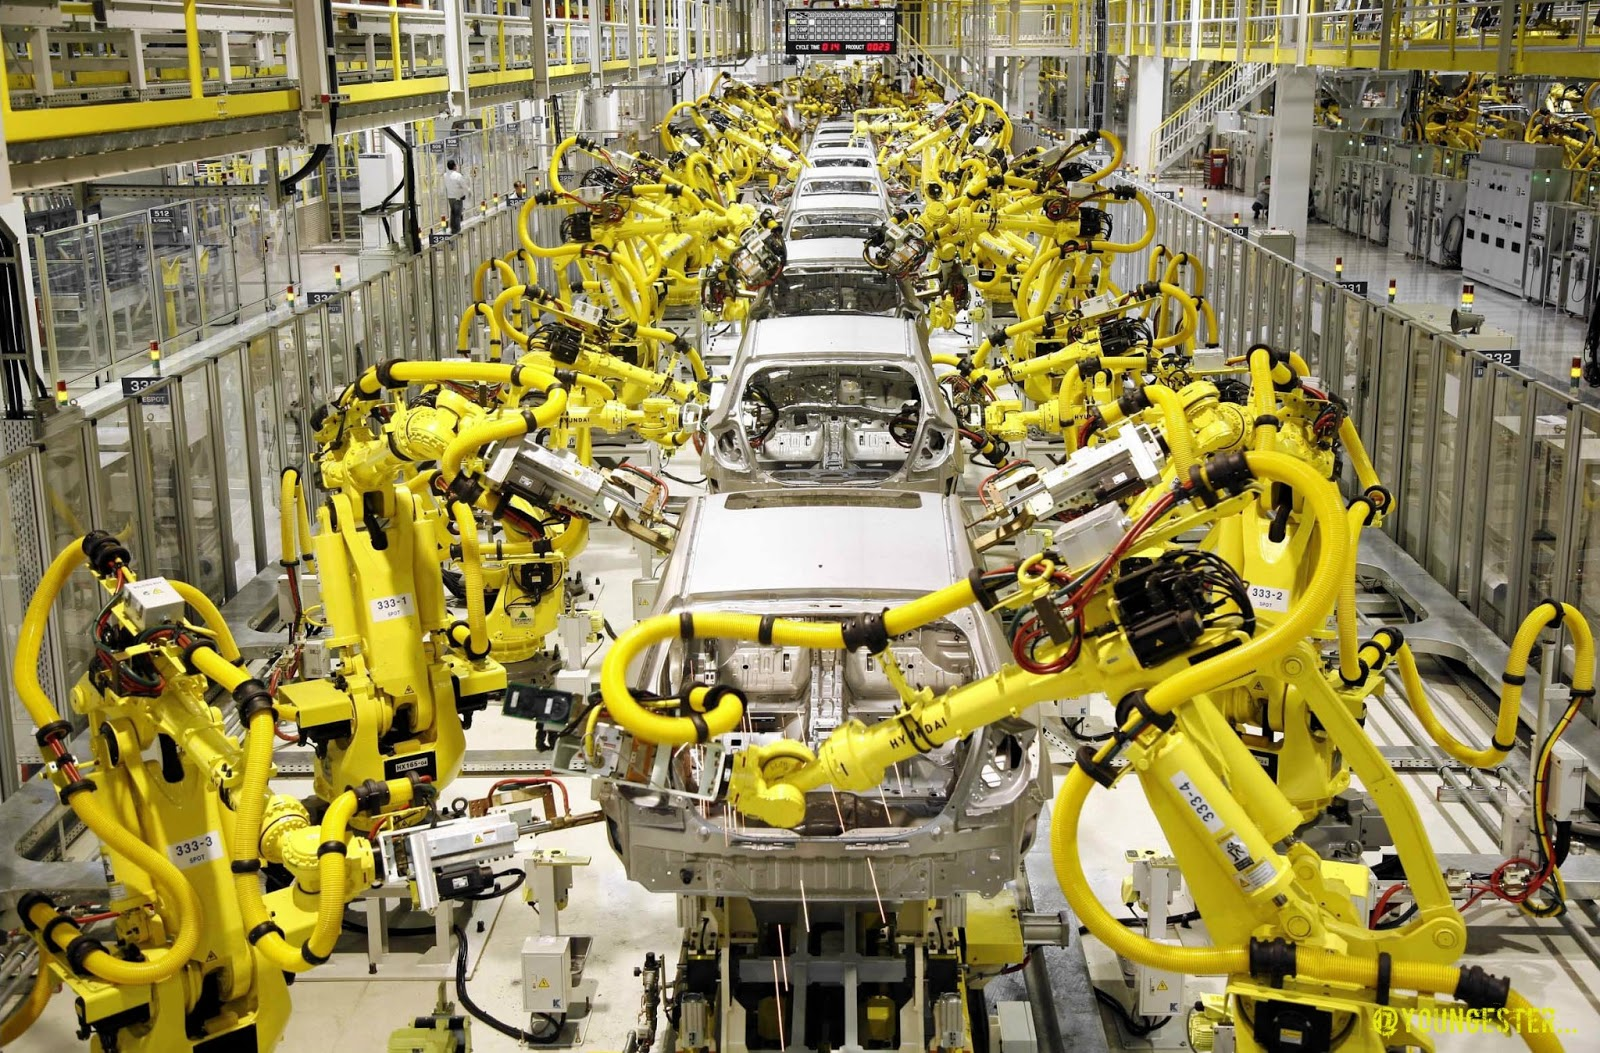
\includegraphics[scale=0.3,width=\textwidth]{Industry}
\end{subfigure}%
\begin{subfigure}{.5\textwidth}
  \centering
  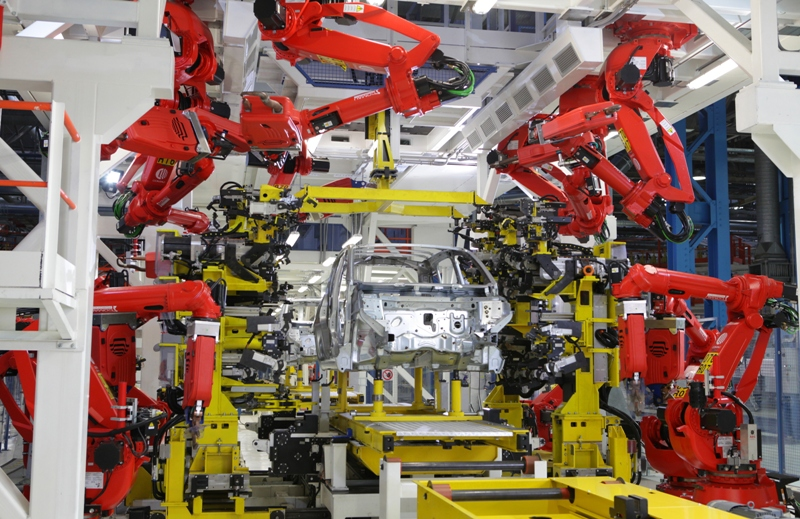
\includegraphics[scale=0.3,width=\textwidth]{Industry2}
\end{subfigure}
\caption{Assembly lines in the automotive industry}
\label{fig:automotive_industry_example}
\end{figure}


\newpage


\section{Literature Review}

This chapter presents a literature review on integrated task an motion planning for multi robot manipulators. Although initial studies have begun since the late 80th, this issue is still a matter of research in academia due to its enormous potential. Moreover as computers getting better implementing a multi-robot planner may be a valuable opportunity for the industry. Our intention is: 1) to get the full picture of these research field 2) to know the current state of the art, and 3) formalizing a standard approach for such a problem.


\subsection{Motion Planning}
\label{section:motion_planning}

Todo: Motion planing for robotic arms

Todo: Collision Checking

We will start with a general description of the problem of planning for multi arms/agents. Lavalle \cite{lavalle2006planning} 
has showed that motion planning problem formulation  is basically identical for single and multi robots, thus theoretically both have the same sampling based nor combinatorial search algorithms. Therefore scaling in the number of DoF is the only parameter affects the search process. For example, planning for 6 manipulators having 6 DoF each results in calculating motion plan for 36 DoF. Examine the most popular motion planners such as RRT \cite{lavalle1998rapidly}, PRM \cite{kavraki1996probabilistic} 
or their more recent variants, we found that it is computationally high to solve (exponential in time). There are two main approaches for calculating motion planning in systems consist of high number of DoF. 


\textit{Centralized Motion Planning} \\
The first (and tentative) is the Centralized Motion Planning in which the total DoF are taking into account when searching for solution. Although computational power is needed (i.e takes time), its pros comes with complete and optimal solution if any.

\textit{Decoupled Motion Planning} \\
Alongside, the second approach Decoupled Motion Planning is more relevant in term of time consuming but lacks the completeness and optimality traits. As listed in \cite{smith2012dual,lavalle2006planning} decoupled planning is categorized into 3 main methods:
	


\begin{enumerate}
  \item $Prioritized~Planning$ (PrP), 
In this approach we sort all the robots by priority and planning an individual path for each robot. Each path is calculated based on the hierarchy obtained by the sorting procedure, such that higher rank is being calculating first. The collision free element acquired by treating the higher ranking robots as a moving obstacles.

  \item $Fixed~Path~Coordination$ (FPC),
This method is divided into 2 parts. At the first stage a path is planned for each individual robot as if its the only robot in the world so that in the second stage all of the paths a getting synchronize by means of timing in order to avoid collisions.

  \item $Fixed~Roadmap~Coordination$ (FRC), 
This strategy extends the FPC by assuming that each robot is guided by a roadmap. This yields a wider set of routes to achieve a single robot goal (instead of one in the FPC). Thus timing of the overall coordination may be more accessible.

\end{enumerate}

Works discussing motion planning for multiple robots often adopt one of the two approaches or else suggests a hybrid solution. A comparison between those approaches is given by Sanchez and Latombe \cite{comparecentralizeddecoupled} using the PRM planning scheme. In this work the authors examined a 36 DoF motion planning problem with each of the approaches described above and with the same path finding technique (SBL \cite{sanchez2002delaying}). Experimental results have shown that the decoupled planning has failed in 30 to 75\% of the trials and among the successful one the time differences had no significant change.


\subsection{Task and Motion Planning}
High and low level planning attributes are "must to have" when designing  an autonomous behaviour in robotics. Each attribute standalone has no capability of getting insights from the big picture of the world: high level plan has to be based on physical properties where low level plan has to be guided by some rule. As of writing this paper the current \textit{state~of~the~art} has no standard formulation for such a binding. For this reason, we aim to give our focus and effort in the area of combining task and motion planning.


\subsubsection*{Task and Motion Planning for Multi Manipulators}
Motion planning for multi-agent robots is an extensive research field consist of many variants. In this work we target to combine Task and Motion Planning for Multi Manipulators (TMPMM) mission. Maybe the main difficulty in such problems is planning for continuous and abstract configuration (states), this because motion planner are not comply with abstract parameters so as task planner don't comply with continuous parameters. TMPMM assignment are separated into 2: the ordinary pick and place task and the cooperative task. 

An interesting work made by Koga and Latombe \cite{koga1994multi} describes a task of moving an object in a world built with obstacles using 3 arms having 6 DoF each. The solution suggested is based on calculating a path for the object while simultaneously check whether it can be grasped by one of the arms. If it reaches a configuration where the grasp is no more valid it search to grasp the object using a different arm and continues with the object's path. This way it's ensures the object continuous motion through a calculated cartesian path while being grasped.



\newpage
\section{Methodology}
%בפרק זה נעבור על הדרך להשגת מטרת המחקר כפי שהוצגה בהקדמה. מכיוון שמטרה זו הינה כללית עלינו להגדיר בצורה ספציפית מהן הבעיות אותן אנו מעוניינים לפתור ולאחר מכן מהם השלבים לפתרונן. לאורך הפרק אנו נעבור תחילה על ההנחות אשר על בסיסן נגדיר מהן הבעיות הפתוחות שאנו מתכוונים לפתור לאחר מכן נדון בדרישות המערכת ובאנליזה שיש לבצע עבור הצעת פתרון כך שבוף הפרק נעבור על הסימולציות והניסויים שנבצע ככלי לבדיקת הפתרון. 

This chapter is about defining the research problems and the ways for solving it. Since the research target (as presented in chapter \ref{section:introduction}) is general, we have to define specifically what are the problems and how to find a solution. Throughout the chapter we will discuss over
\begin{inparaenum}[\itshape a\upshape)]
\item the definition that is used as a basis to define a research problems
\item the system requirements for a solution
\item the methods for analysing a solution 
and
\item the simulation/experiments that will evaluate a solution performance.
\end{inparaenum} 
 

 


\subsection{Research Problem Description}
\label{section:problem_description}
%על מנת להגדיר בצורה ברורה יותר מהן הבעיות אותן נפתור תחילה נגדיר את הנחת הבסיס. אנו נשתמש בעובדה כי ברוב הזרועות התעשייתיות בסיס הזרוע הינו סטטי ולכן כשמדובר בקבוצה של זרועות המרחקים בין הבסיסים קבוע, עובדה זו מובילה אותנו להנחת הבסיס 
%של המחקר

In order to define more clearly what problems are we going to solve, first we will specify the research basic definition. We will use the fact that the majority of industrial robotic arms are statically based and so a group of arms have fixed distances between their bases. This fact leads us to the next definition:

\begin{definition} \label{def:basic_def}
A configuration set of robotic arms is given such that:
\begin{enumerate}
\item[a)] The arms links length, joint orientation and joint limitation is known.
\item[b)] The arms base position is known.
\end{enumerate}
\end{definition}

To complete a problem description, we will have to specify what objects are we going to use and the action which the arms will apply. The overall package of arms, objects and actions are the building stones of the next 4 problems:

\subsubsection*{Problem 1: Pick and Place of Single object by a Set of Robotic Arms}
%כאן, תיאור הבעייה נתון ע"י אוסף של זרועות רובוטיות ביחד עם אובייקט יחיד כך שהמטרה היא להעביר את האובייקט ממיקום התחלתי למיקום סופי מוגדרים מראש. ומכיוון שניתן להעביר את האובייקט ע"י הזרועות בלבד לנסח את סט ההנחות הבא:
%סט ההנחות הבא:
%קונפיגורציית הזרועות נתונה
% המיקום ההתחלתי והסופי של האובייקט ידועים וממוקמים בסביבת עבודה של זרוע אחת לפחות 
 
Here, the problem description is given by a set of robotic arms together with a single object such that the task is to move the object from its initial position to a predefined goal. Knowing that only arms are able to manipulate an object we can define the next assumptions:
\begin{itemize}
\item The initial configuration of the arms set is known.
\item The initial and final position of the object in known and located at a workspace belongs to (at list) one of the arms.
\item Only a single arm can grasp the object at a time. 
\item There are two types of obstacles: the arms themselves and the object.
\end{itemize}
In practice the difficulty arise when a single arm is not capable of completing the task alone and the solution gets a form of series of arms preforming pick and place operation (i.e transferring the object between themselves). This problem expose a number of open question:
\begin{enumerate}
\item What is the sequence of arms which will complete such a task.
\item What are the positions along the object path where a transfer happens.
\item What is the collision free trajectory of each arm throughout the sequence.
\end{enumerate}


\subsubsection*{Problem 2: Pick and Place of Multiple objects Simultaneously }
This problem expands problem 1 above such that the assignment is to move multiple objects from one place to a predefined goal using robotic arms only. This problem adds complexity to the overall system and expose the next assumptions:
\begin{itemize}
\item The initial configuration of the arms set is known.
\item The initial and final position of all of the objects in known and located at a workspace belongs to (at list) one of the arms.
\item The final configuration of all of the objects is defined without collisions.
\item A single arm cannot manipulate more than one object simultaneously.
\item Only a single arm can grasp an individual object at a time. 
\item There are two types of obstacles: the arms themselves and the objects.
\end{itemize}

%במבט ראשון ניתן לפתור בעייה זו בשני שלבים כך שדבר ראשון משתמשים בפתרון של בעיה 1 עבור כל אובייקט בנפרד ולאחר מכן ניתן לתזמן את סדר התנועה כך שלא יפגעו ההנחות. פתרון מסוג זה אומנם אפשרי אבל אינו מנצל את מלוא היכולות של המערכת העשויים להביא לפתרון מהיר יותר ולכן אנו נשארים עם אותן שאלות פתוחות כמו אלו שבבעיה 1.

At first look, this problem can be solved using \textit{prioritize planning} principle; a solution for problem 1 is obtained for each object individually, next an execution scheduling process is maintained in order to avoid conflicts. Although it is an applicable solution it does not exploit the full capabilities of such a system which could handle a faster solution. Thus, the same open question as of problem 1 remained.

\begin{enumerate}
\item What is the sequence of arms that will manipulate each object.
\item What are the positions along the each object path where a transfer happens.
\item  What is the collision free trajectory of each arm throughout the sequences.
\end{enumerate}
  
\subsubsection*{Problem 3: Pick and Place of Single/Multiple objects in Environments with Obstacles}
This problem is defined the same way as problem 1 and 2 (i.e as a single or multi object manipulation problem), except that it defined with a new type of obstacles (static nor dynamic). Thus, the last assumption in each problem list is changing as follows:
\begin{itemize}
\item The obstacles geometry, type and position are known.
\item There are three types of obstacles: The arms themselves, the objects and the environmental obstacles.
\end{itemize} 
The problem of cluttered environment adds complexity to the system such that it limits the motions of arms nor the positions of the transfer points. Hence, it is mainly affects the motion planning part of the total planning scheme. 

\subsubsection*{Problem 4: Pick and Place of Single/Multiple objects with Non-Homogeneous Team of Robotic Arms }
In the case of non-homogeneous teams of robotic arms we depict a the same problem of moving an object by a series of arms, only now there are different kind of arm. A warehouse management robot team would be a good application where heavy lifting robotic arms are needed for manipulating plates and a light lifting robotic arms are needed for loading/dispersing boxes on top of the plate. In contrast to the scenarios of problem 1-3, here we let a single arm to manipulate number of objects at a time (as long as the objects are organized in a way that enables to grasp). 




\subsection{Algorithm Development}
\label{section:algorithm_development}
The problems described in section \ref{section:problem_description} have both decision and motion planning attributes. Each attribute standalone has a formal approach for solving it but lacks the other skills. Still, in order to solve these problems a 2 phases solution is required:

\begin{enumerate}
\item[(phase 1)] A high level task plan with a general purpose aimed to find a sequence of arms that will transfer an object from initial to goal positions. 
The idea behind this phase is to find a series of "arm indexes" where the object is being passed from one arm to the next such that the last arm will place the object at it's target.


\item[(phase 2)] A low level motion plan with a general purpose aimed to actually calculate a collision free trajectory for each step of the sequence. This is a more physical phase where the joint/work spaces of all of the arms are taken into account when calculating such a trajectory. The collision free refers for an arm that is transferring an object towards the next arm in the series (or toward the object's goal).

\end{enumerate}

The two phases are coupled due to the fact that any logical sequence of arms is based on geometric properties, for example any 2 following arms should share a gripping position of an object (in global coordinates) in order to transfer it between themselves. Having this fact in mind we understand that our algorithm first objective is to combine the two phases above by searching for applicable sequence it terms of kinematic feasibility. 
Having a feasible sequence applies for being able to grasp an object at each step by a different arm, this is literally interpreted as a state where a configuration of a single arm was set. This notion leads us to our second algorithm objective which is to calculate a transition function between those states. Here, a transition function is a motion plan as detailed in phase 2 above and this is a key feature for success in such algorithm.


As for our third objective is to be able to use this algorithm for a maximal number of arms nor objects. This is a high priority goal which makes a major contribution for such a scenarios. The trade off for large scale planning is of-course linked to computation time of the algorithm. From this perspective, We expect the weakness of the algorithm at the motion planning phase. As shown in section \ref{section:motion_planning} applying a \textit{centralized} motion planning method on a system with high number of DoF will doomed to time-out before having a solution.  


\subsection{Algorithm Analysis}
In order to validate the capabilities of any algorithm we should assess two major specifications:

\begin{enumerate}

\item[\textbf{Completeness}] This first parameter states for knowing whether a solution exist and as long as one exist if the algorithm can find it.

\item[\textbf{Complexity}] This parameter has a direct link to solutions computation time. In most cases this parameter estimates the maximal operation to do in order to find a solution (if any). In practice complexity tend to over estimate the computation time of a solution which actually much more faster. Thus, to get a realistic point of view about how good is our algorithm we should compare its performance against other techniques.


\end{enumerate}




\subsection{Simulation and Experiments}
\label{section:sim_and_exp}

Any design of planning algorithm that implements phase 1 and 2 of section \ref{section:algorithm_development}) will be tested under simulation and experiments, this in order to present its capabilities of displacing an object using multiple arms. The simulation code will be written under MATLAB environment which later on will be re-written with c++ in order to handle the experiments under GAZEBO/ROS framework. Although GAZEBO is a 3D simulation it holds behind a dynamics engine that calculates the physics of solid parts in terms of equation of motion and interacting forces (between two parts). This means GAZEBO can be used as a experiments environment where we can test scenarios consist of as many robot arms as we need. 

The objective of these simulation is to preform a parametric inquiry which aimed to check the influence of a single parameter on the overall performance. The parameters that interesting us are as follows:

\begin{enumerate}
\item The number of robotic arms in a setup.
\item The total percentage of the shared workspace of an arm.
\item The number of joints/links having a single arm.
\end{enumerate}


Throughout the research our target is to apply this inquiry over the problems listed in \ref{section:problem_description}, thus for each of these problems we will have to build a different setup. Table \ref{table:experiment_setups} shows four different setups that will be tested on each problem. As detailed, column 2 represents the number of arms in a setup, column 3 represents the percentage of workspace shared between any couple of arms and column 4 represents the number of DoF in each arm.  
\begin{table}[t]
\begin{center}
\begin{tabu} to 1\textwidth { | X[-2m c] || X[c m] | X[c m] | X[c m]| }
%\begin{tabular}{ |c||c|c|c|  }
 \hline
 Setup Index & Number of Arms in a Setup & Percentage of Workspace Sharing & Number of DoF in a single arm\\ 
 \hline
 \#1         & 3                         & 20 & TBD \\
 \#2         & 3                         & 80 & TBD \\
 \#3         & 10                        & 20 & TBD \\
 \#4         & 10                        & 80 & TBD \\
 \hline
\end{tabu}
%\end{tabular}
\caption{4 different setups to handle a parametric inquiry over the research problems}
\label{table:experiment_setups}
\end{center}
\end{table}
In fact, any change of a setup parameters will change the output of a planning algorithm such that we can estimate what are the factors that influencing on:
\begin{enumerate}
\item The total task operation time.
\item The overall configuration size.
\item The computation time.
\item How many robotic arms can be used.
\item What type of arms can be used.
\item How "dens" the arms are located.
\end{enumerate}

Also, these setups are interpreted as both two or three dimensional problem, although in general a 2D problem may be more easy to solve it is not the often case here (See Appendix............). Still, the procedure for testing a problem in our research will be first simulation and experiments over a set of planner robotic arms and next simulation and experiments on a set of spatial robotic arms (The number of arms and the percentage of shared workspace remains the same). 

%
%\subsubsection*{Application of Problem 1}
%This is our simplest problem which made to stand for a basic case that an algorithm will have to handle. Moreover, applying an algorithm that solves this case means a proof of concept for a more general approach. Thus, implementing a system setup as detailed in table \ref{table:experiment_setups} is a straight forward task. As the nature of simulation is to be held on computers the advantage here is to run as many simulations as we need 


ToDo: explain position controlled
  

\newpage
%
\section{Preliminary Results}


\subsection{Case Study}
For our case study we want to analyse the problem of pick and place a movable object throughout a workspace containing a number of robotic arms. We represent the world using a cylinder (i.e beer can) as an object together with \textit{m} grippers connected to \textit{m} statically based robotic arms which allowed to move on a planner surface (i.e table). An example of a case consist of 5 arms is represented in figure \ref{fig:case_study}.

\begin{figure}[htb]
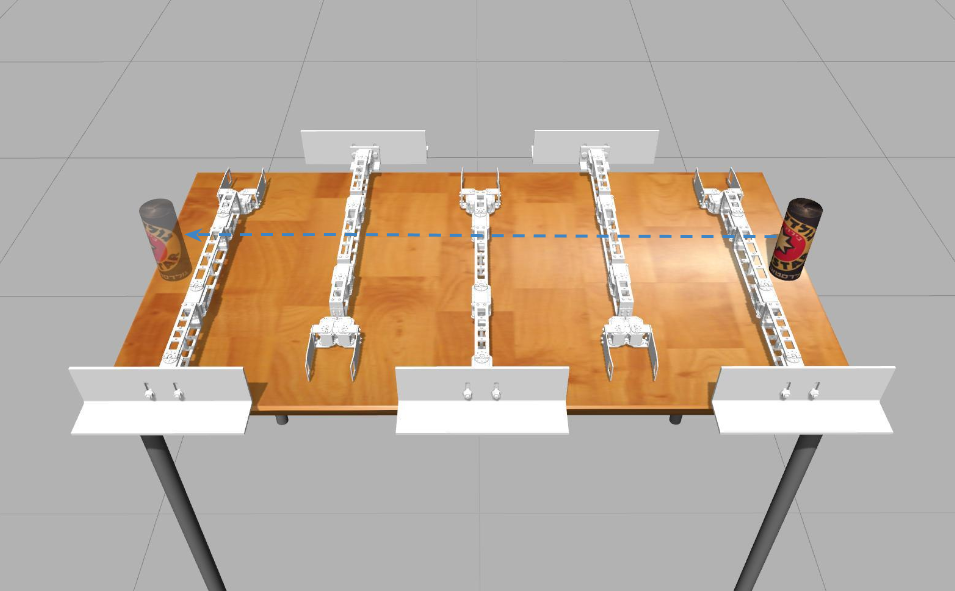
\includegraphics[scale=0.3,width=\textwidth]{5arms}
\centering
\caption{Case study Visualization} \label{fig:case_study}
\centering
\end{figure}


\subsection{Problem Formulation}
In this work our intention is to engage a single object pick and place problem using multi manipulators. We will handle the next symbols description for our problem statement. A manipulator will denoted as $A^{i}$ (the i'th parameter means the manipulator index) and an object as \textit{B}. We assume to have an overall of \textit{m} manipulators  $\mathcal{A}=\{A^{1},A^{2},\dots,A^i \dots,A^{m}\}$ and a single movable object. Furthermore we assume that each $A^i$ holds a workspace $W^{i}$ and a configuration space $C^{i}$ such that 
the Forward Kinematics (FK) is mapping $W^i$ from $C^i$ ($FK:C^i\rightarrow W^i$). Hence, the feasible workspace of the object will be then $\mathcal{W}^B=\{W^{1} \cap W^{2} \cap \dots  W^{i} \dots \cap W^{m} \}$ the overall \textit{configuration space} of the arms will be $\mathcal{C}^A=\{C^{1} \times C^{2} \times \dots  C^{i}  \dots \times C^{m} \}$  and the corresponding arm \textit{workspace} $\mathcal{W}^A=\{W^{1} \times W^{2} \times \dots  W^{i}  \dots \times W^{m} \}$ . 


For the purpose of consistency with \cite{koga1994multi,koga1992} we will presume the terminology of \textit{transit-path}, \textit{transfer-path} and \textit{manipulation-path} as follows:
\begin{itemize}
\item[\textit{transit-path}] is a path that describes a motion of an empty arm (i.e not grasping any object). We will use this term to represent a path of an arm which avoids collision with other arms or actually moving toward an object in order to grasp it.

\item[\textit{transfer-path}] is a path that describes a motion of an arm that is grasping an object within its gripper. We will use this term to represent a path of an arm that manipulates an object.

\item[\textit{manipulation-path}]  is a sequence of alternating \textit{transmit} and \textit{transfer} paths. We will use this term to represent a sequence of arms the moves an object from initial to goal positions.

\end{itemize}
Next, consider the following problem input:


\begin{itemize}
\item A set of $m$ robotic arms. 
\item Initial and goal positions of an object $B^{init},B^{goal} \in \mathcal{W}$
\end{itemize}
our objective is to find a \textit{manipulation-path} along which the object could be transferred according to input requirements. By definition each manipulation path is constructed by a sequence of \textit{Tspace} paths $\mathcal{T}^A=\langle T^{1},...,T^k, ...,T^n\rangle$ where $T^k \in \mathcal{W}^A$. In addition, each \textit{Tspace} path is derived by applying the FK rule on a sequence of $Cspace$ path. Therefore the corresponding \textit{Cspace} sequence of $\mathcal{T}^A$ resemble as $\mathcal{Q}^A=\langle Q^{1},...,Q^k, ...,Q^n\rangle$ where $Q^k \in \mathcal{C}^A$. This observation shows that any solution is obtained by calculating $\mathcal{Q}^A$ such that the equivalent $\mathcal{T}^A$ preforms a desired manipulation path. It is noteworthy that each $T^k$ is holding a $transit$ path for the entire arms (to operate in parallel) except one that holds a pair of $transit$ and $transfer$ paths for the actual manipulation.


\subsection{Planning Logic}

We let $\mathcal{T}^B$ be the object absolute path (i.e from initial to goal positions) such that $\mathcal{T}^B \in \mathcal{W}^B$, next we consider any $k$ element as a sub-task operation that moves the object along a portion of $\mathcal{T}^B$. Hence, we can reason that $\mathcal{T}^B$ is built up by a sequence of \textit{work-space} paths each handled on the $k$'th sub-task by a different arm, thus $\mathcal{T}^B = \langle T^B_1,...,T^B_k,...,T^B_n \rangle $. 

We define that object is restricted to move only when it is gripped, this aims the search 
to find a particular sequence of arms $S(k) \subset \mathcal{A} \mid [k=1..n] $ that will do the feasible manipulation job. Recall that any solution is represented by a sequence of $T^k$'s where each holds a path for the total arms. This means that $T^k$ is built by the set of $Tspace$ path of each individual arm $T^k = \{ T^{k,1},...,T^{k,i},...,T^{k,m} \}$. The resulted conclusion is an essential connection extracted between $\mathcal{T}^A$ and $\mathcal{T}^b$ such that for any $k$: $T^B_k = T^{k,S(k)}$.

We'll denote a $transfer~point$ as a position where any $T^B_k$ starts or ends (including $B^{init}$ and $B^{goal}$). Tentatively any $transfer~point$ located where an object is grasped or released by all of the arms in $S$. Any sequence $S$ consist of $n$ arms will have to pass through $n+1$ $transfer~points$ series $tp$. Assuring this condition is given by forcing any $T^{k,S(k)}$ to include $tp(k)$ and $tp(k+1)$ along their path. A summary of the general conditions for a valid $\mathcal{T}^A$ is as follows:
\begin{equation}
\label{eq:kinematic-feasible}
        \forall T^{k}: \{\exists Q^{k} \mid (T^{k} = FK(Q^{k})\} 
\end{equation}

\begin{equation}
\label{eq:consistant-sequence}
        \forall T^{k,S(k)}: \{ tp(k),tp(k+1) \in T^{k,S(k)}  \}
\end{equation}

\begin{equation}
\label{eq:no-collision}
        \forall T^{k}: \{ T^{k,i} \cap T^{k,j} = \emptyset \mid i,j=1..n~;~i\neq j \}
\end{equation}
where equation \ref{eq:kinematic-feasible} referring to kinematic feasible path, equation \ref{eq:consistant-sequence} is responsible for applicable sequence in terms of pick and place positions and equation \ref{eq:no-collision} imposing for having no collisions.





\subsection{Planning Process}
Recalling the work of Koga and Latombe \cite{koga1994multi}, it is shown that the object's world trajectory is the governing law when it comes to determine which is the grasping arm at any time. On the contrary we wish to give another perspective for the problem. Our guiding rule comes from shared workspaces of the arms. We are using the fact that any $transfer~point$ is located only in one of the shared workspaces and consequently $\mathcal{T}^B$ must pass through them. 

\begin{figure}[t]
    \centering
    \begin{subfigure}[b]{0.4\textwidth}
        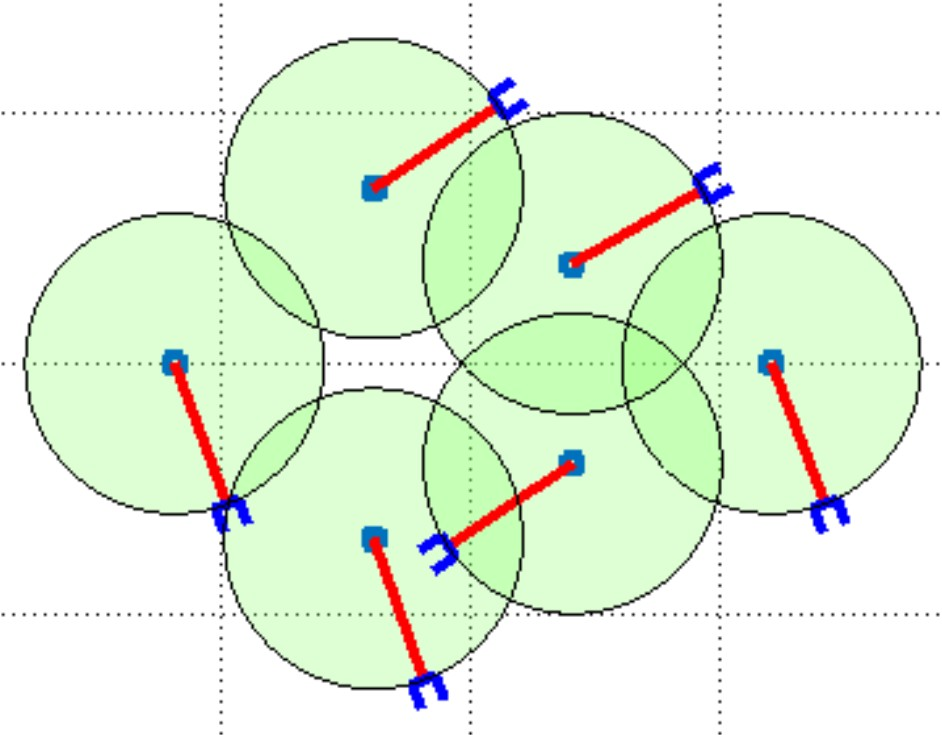
\includegraphics[width=\textwidth]{general_configuration}
        \caption{general configuration}
        \label{fig:general_configuration}
    \end{subfigure}
    ~~~~
    \begin{subfigure}[b]{0.4\textwidth}
        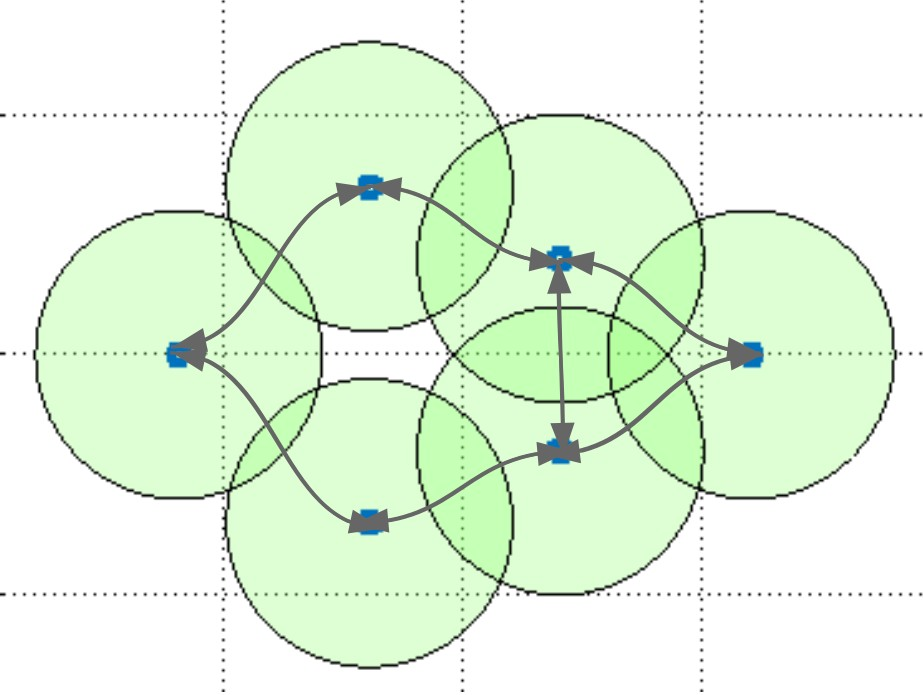
\includegraphics[width=\textwidth]{generated_graph}
        \caption{phase 1: generated graph}
        \label{fig:generated_graph}
    \end{subfigure}  
    
    \begin{subfigure}[b]{0.4\textwidth}
        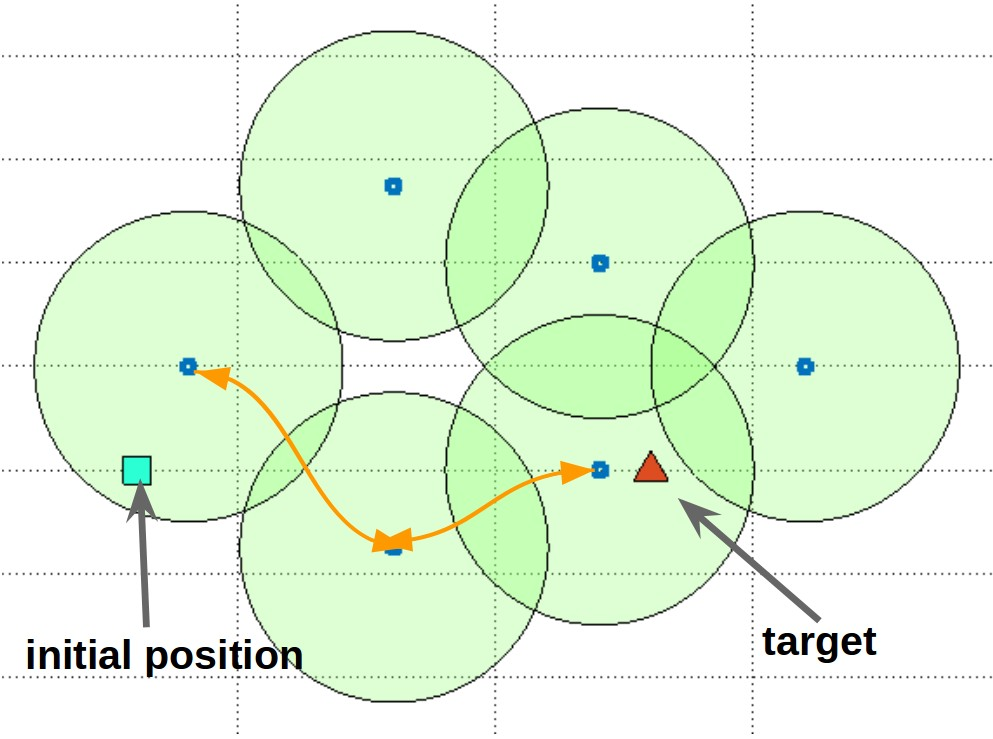
\includegraphics[width=\textwidth]{task_assignment}
        \caption{phase 2: Graph shortest path based on task properties }
        \label{fig:task_assignment}
    \end{subfigure}
    ~~~~
    \begin{subfigure}[b]{0.4\textwidth}
        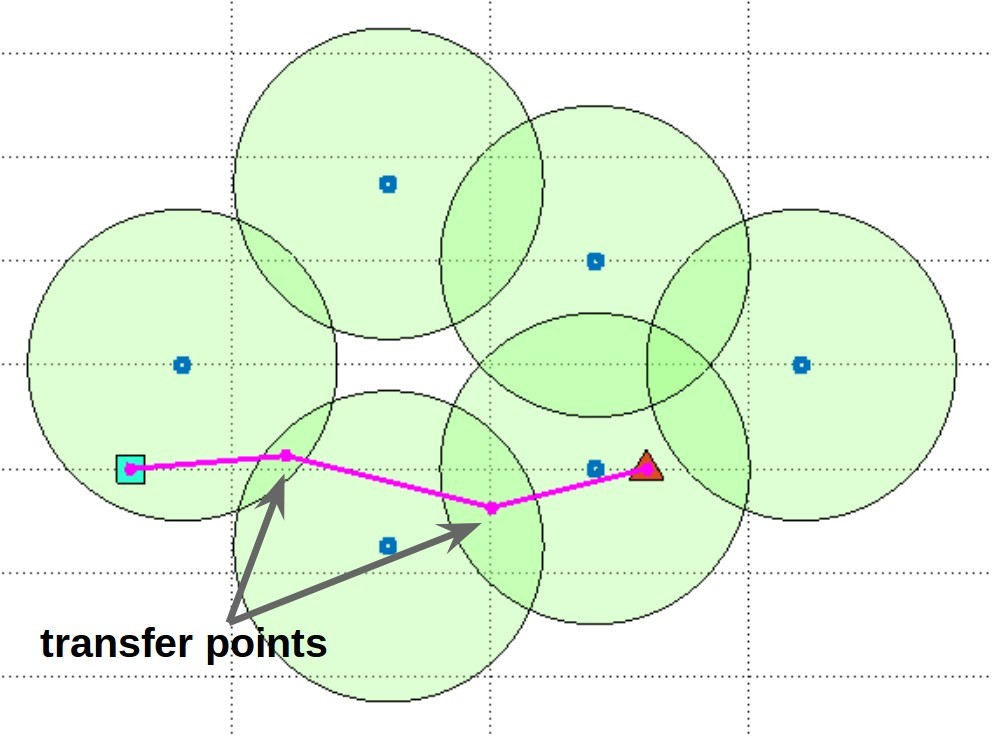
\includegraphics[width=\textwidth]{transfer_points}
        \caption{phase 3: calculating transfer points}
        \label{fig:transfer_points}
    \end{subfigure}
    \caption{Generating a sequence of arms and transfer points}\label{fig:animals}
\end{figure}

\subsubsection*{Search for Arm Sequence and Transfer Points}

One of the key component of our work is find any pair of arms sharing together a part of their workspace such that $W^i \cap W^j \neq \emptyset$, this fact gives an insight for any transfer that could appear. The easiest way to represent this data is by a graph where a node represent an arm workspace and an arc represents a shared workspace (between two arms/nodes). It means that a world consist of $n$ arms is interpreted by a graph with $n$ nodes where arcs are added on a second phase by checking any possible combination of shared workspaces. The generation of this graph will tentatively be called the $connectivity~graph$.

By attributing the initial and goal position of the object to one of the arms $Tspace$ we can reason about the starting and final node in the $connectivity$ $graph$. 
At this point, any graph search would give a solution with a form of a sequence of arms $S = \langle A^{first},...,A^k,...,A^{last} \rangle$ connected by their shared workspaces such that:
\begin{equation}
B^{init} \in W(A^{first})\mid A^{first}\equiv S(1)
\end{equation}
\begin{equation}
B^{goal} \in W(A^{last})\mid A^{last}\equiv S(n)
\end{equation}
\begin{equation}
W(A^{k})\cap W(A^{k+1})\neq \emptyset \mid A^{k}\equiv S(k)
\end{equation}
After generating \textit{S} the next task is to determine the position of a single \textit{transfer point} located in each shared WS. To do so a linear programming method will be used to minimize the total length accepted by connecting any pair of following \textit{transfer point} with a straight line.


\subsubsection*{The Search Algorithm}
To generate an actual sequence that will apply the condition as in equations \eqref{eq:kinematic-feasible}-\eqref{eq:no-collision} we will have to go through the steps as written in algorithm \ref{alg:main-loop}. The rationale behind this algorithm is first to find a sequence of arms $S$ together with a series of $transfer~points$ $tp$ that will settle with equation \eqref{eq:consistant-sequence} (lines 1-5). Next, when $S$ and $tp$ was determined the guidelines for a motion plan was resolved, thus the second phase of the algorithm was launched (line 6) in order to calculate the sequence path that meet equations \eqref{eq:kinematic-feasible} and \eqref{eq:no-collision}. 

\begin{algorithm}
\caption{Main Loop} \label{alg:main-loop}
\begin{algorithmic}  [1] % the [1] is for numbering
\REQUIRE $B^{init},B^{goal},\mathcal{A},q^{init}$
\ENSURE $traj$
	\STATE $cg\leftarrow GenerateConnectivityGraph(ws)$
	\STATE $W^{first}\leftarrow $ find($W^{first}$ such that $B^{init}\in W^{first}$)
	\STATE $W^{last}\leftarrow $ find($W^{last}$ such that $B^{goal}\in W^{last}$)
	\STATE $S\leftarrow$ BFS$( cg,W^{first},W^{last})$ // generate ws sequence
	\STATE $tp\leftarrow CalcTransferPoints( S,B^{init},B^{goal} )$
\STATE $\mathcal{T}^A \leftarrow CalcSequenceTrajectory( S,tp,q^{init})$
\end{algorithmic}
\end{algorithm}








\subsubsection*{Calculating Sub-Task Path}
As stated, at this stage our goal is to calculate the arms path for each phase of the \textit{manipulation-path} represented by $\mathcal{T}^A$. We assume that each phase includes the following input parameters (and that the initial configuration of the total arms is known):

\begin{itemize}
	\item Index of the moving arm.
	\item Initial and goal positions of the arms gripper
\end{itemize}

These parameters directs us to find a motion planning solution for a multi robot system. As mentioned in section \ref{section:motion_planning} there is no formal strategy for calculating optimal nor complete trajectory for multi robots except for using \textit{centralized} methods that suffers from exponential complexity. The pattern that we will next describe is a method that is designed to find a solution oriented for robotic arms but may still be used for other systems. 

The fact that a \textit{centralized} method includes complete and optimal attributes is that it can handle local minima's (same as A*). Lack in such feature resolved in having no reasoning when: robot 2 obstructs the path of robot 1 where actually robot 1 obstructs the path of robot 2 that should clear the path for robot 1. A simple illustration is shown in figure \ref{fig:initial_configuration} with a case of 2 robotic arms having 1 DoF each. The task here is to move arm \#1 to the dashed line. Trying to do so with applying any motion plan on arm \#1 only will result with "no solution" answer. It is obvious that arm \#2 needs to clear the way and the only option is to move counter-clockwise (moving clockwise is impassible due to the obstacle). 



\begin{figure}[t]
    \centering
    \begin{subfigure}[b]{0.3\textwidth}
    		\centering
        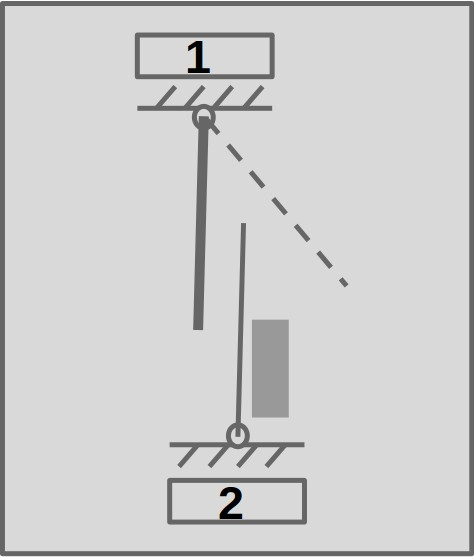
\includegraphics[width=0.8\textwidth]{initial_configuration}
        \caption{Initial configuration of the arms, goal of arm \#1 is dashed \\ }
        \label{fig:initial_configuration}
    \end{subfigure}
    ~
    \begin{subfigure}[b]{0.3\textwidth}
    		\centering
        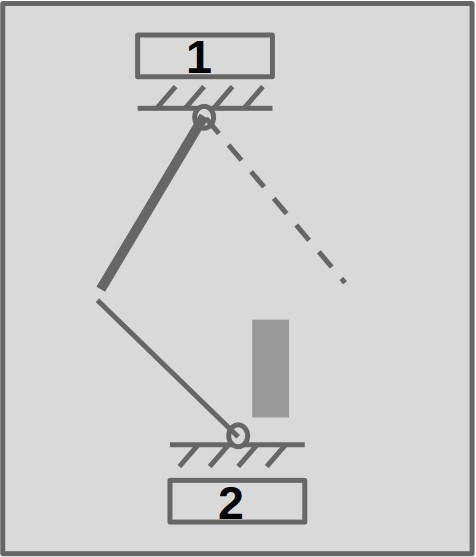
\includegraphics[width=0.8\textwidth]{breaking_point}
        \caption{A configuration of a "breaking point" from which the goal is reachable for a single arm task}
        \label{fig:breaking_point}
    \end{subfigure}  
    ~
    \begin{subfigure}[b]{0.3\textwidth}
    		\centering
        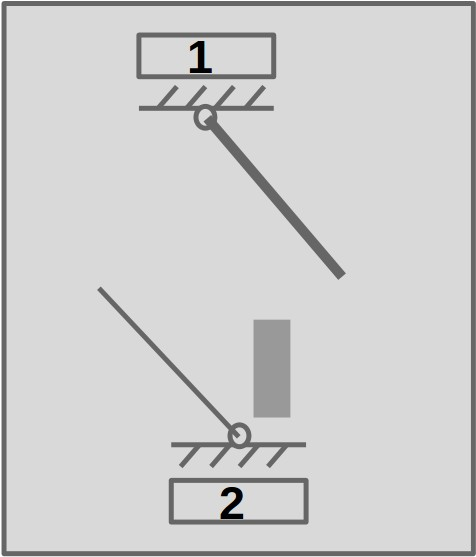
\includegraphics[width=0.8\textwidth]{final_configuration}
        \caption{Final configuration: goal achieved \\ \\}
        \label{fig:final_configuration}
    \end{subfigure}

    \caption{A multi arm problem configuration consist of 2 arms with 1 DoF each together with an obstacle (grey rectangle) that limits arm \#2 motion. In order to acheive the goal (figure c) a breaking point (figure b) must be acheived first. }\label{fig:local_minima_example}
\end{figure}




\section{Preliminary Results}

Over this chapter we will describe our proposed solution for the multi arms manipulation planning problem with reference to the first problem in \ref{section:problem_description}. A two dimensional illustration of such a problem is given in figure \ref{fig:case_study}. As introduced, this scenario is an example of a setup built by 5 statically based robotic arms together with an object displacement assignment. As detailed in section \ref{section:sim_and_exp} a similar scenarios varied by the number of arms, number of DoF and the percentage of shared workspace will be examined. Our algorithm objective is to give an automatic generation of a sequence of arms (and motions) for any given scenario/setup.
 
\begin{figure}[htb]
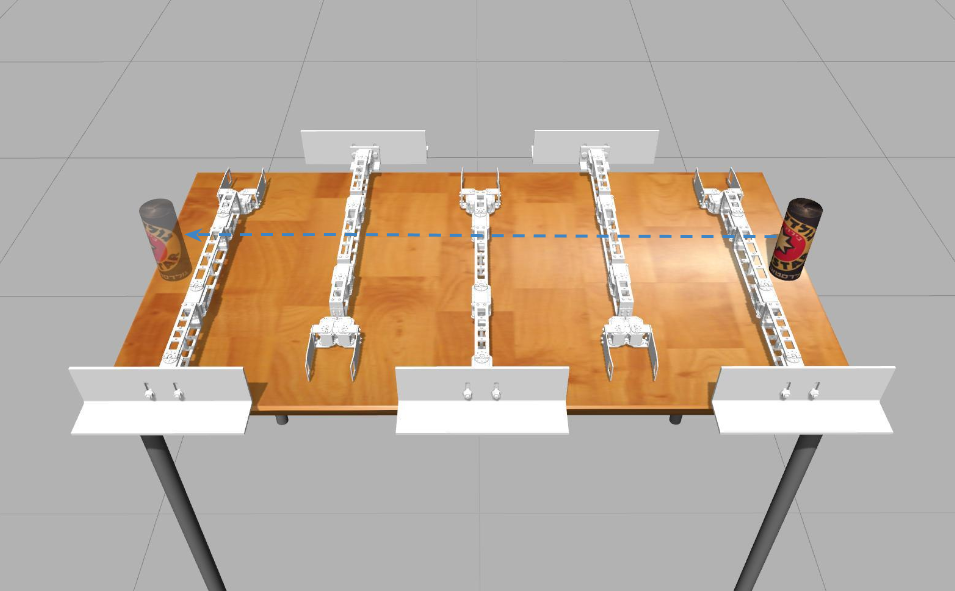
\includegraphics[scale=0.3,width=\textwidth]{5arms}
\centering
\caption{A setup illustration of 5 robotic arms together with a single object} 
\label{fig:case_study}
\centering
\end{figure}


\subsection{Problem Formulation}
In this work our intention is to engage a single object pick and place problem using multi manipulators. We will handle the next symbols description for our problem statement. A manipulator will denoted as $A^{m}$ (the $m$'th parameter means the manipulator index) and an object as $B$. We assume to have an initial configuration given by $M$ manipulators  $\mathcal{A}=\{A^{1},A^{2},\dots,A^m, \dots,A^{M}\}$ together with a single movable object. Furthermore we assume that each $A^m$ is given by
\begin{inparaenum}[\itshape a\upshape)]
\item configuration space $C^{m}$ which represents the space of the arm joints value $c^{m} = \begin{bmatrix} q^{m,1} & q^{m,2} & \dots & q^{m,n} & \dots & q^{m,N} \end{bmatrix}^T$ where $q$ expresses a single DoF, and
\item a workspace $W^m$ which represents the space of the arms gripper positions $w^m= \begin{bmatrix} x^m & y^m & \theta^m \end{bmatrix}^T$ in global coordinates.
\end{inparaenum}  
A mapping function of $W^m$ is given by the Forward Kinematics (FK) rule where $FK:C^m\rightarrow W^m$. Thus, the full state of the system is given by the configuration space of all of the arms $\mathcal{C}^A=\begin{bmatrix} C^1 & C^2 & \dots & C^m & \dots & C^M\end{bmatrix}^T$. Next, for keeping consistency with \cite{koga1994multi,koga1992} we will presume the terminology of \textit{transit}, \textit{transfer} and \textit{manipulation} paths as follows:
\begin{itemize}
\item[\textit{transit-path}] is a path that describes a motion of an empty arm (i.e not grasping any object). We will use this term to represent a path of an arm which avoids collision with other arms or actually moving toward an object in order to grasp it.

\item[\textit{transfer-path}] is a path that describes a motion of an arm that is grasping an object within its gripper. We will use this term to represent a path of an arm that manipulates an object.

\item[\textit{manipulation-path}]  is a sequence of alternating \textit{transmit} and \textit{transfer} paths. We will use this term to represent a sequence of arms the moves an object from initial to goal positions.
\end{itemize}
Next, consider the following problem input:
\begin{itemize}
\item A set of $m$ robotic arms. 
\item Initial and goal positions of an object $B^{init},B^{goal}$
\end{itemize}
Our objective is to find a \textit{manipulation-path} along which brings the object to its goal configuration. By definition each \textit{manipulation path} is constructed by a sequence of arms $\mathcal{S} = \langle s^1,s^2,\dots,s^k,\dots,s^K \rangle$ preforming a \textit{transfer paths}, where $s^k$ represent an arm index and $K$ is the number of arms in $\mathcal{S}$. As each arm of the sequence is identified with a $transfer$ action it holds a configuration space path noted as $Q^k$ (where $Q^k \in C^{\mathcal{S}(k)}$). Now, we can define a sequence of paths $\mathcal{Q}$ for each step of $\mathcal{S}$ such that $\mathcal{Q} = \langle Q^1,Q^2\dots,Q^k,\dots,Q^K \rangle$. Here, each $Q^k$ represent a path for the corresponding arm $s^k$.  

Practically, any execution of $\mathcal{S}$ "as is" may not be a accomplished due to the configuration of the other arms that possibly obstructing the path. As used in \cite{koga1994multi} a straight forward solution is obtained by moving the obstructing arms to a predefined non-obstructive location. This solution is less likely to succeed in 2D problem, especially on setups with high percentage value of the arms shared workspace. To overcome this issue any $Q^k$ path should be coordinated with a \textit{transmit} paths of the arms that are not transferring the object. Thus, in order to move a single arm a full state path is constructed as a subset of $C^A$. This eventually re-defines $Q^k$ with a second index such that $Q^k = \begin{bmatrix} Q^{k,1} & \dots & Q^{k,m} & \dots & Q^{k,M} \end{bmatrix}^T$ where $Q^{k,m}$ represent the $A^m$ path over the $k$ step. In summary, a solution is formulated with the following parameters:
\begin{enumerate}
\item A sequence of $K$ arms indexes $\mathcal{S}$ that represent which is the $transfer$ arm at each step.
\item A sequence of $K$ paths $\mathcal{Q}$ that represent the motion of all the arms at each step of $\mathcal{S}$ (i.e the \textit{manipulation} path).  
\end{enumerate}

\subsection{High Level Planning}

As detailed, a \textit{manipulation} path is built by a sequence of pick and place operations which in nature defines a sequence of subtasks. Thus, for convenience we will use the term subtask to denote the $k$'th procedure in $\mathcal{Q}$. Being able to solve each subtask separately simplifies the problem to a single arm pick and place solution. Still, this advantage makes no guaranties for solving the overall task unless a binding condition will be made between two following subtasks. Such a criteria is built by the \textit{transfer point} terminology.  

We let $\mathcal{T}^B$ be the object absolute path from its initial to goal position. By definition, each subtask moves the object along a portion of $\mathcal{T}^B$. Hence, we can reason that $\mathcal{T}^B$ is built up by a sequence of \textit{work-space} paths each handled on the $k$'th subtask by a different arm, thus $\mathcal{T}^B = \langle T^{B,1},...,T^{B,k},...,T^{B,K} \rangle $. We will denote a \textit{transfer point} as a position where any $T^{B,K}$ starts or ends. Tentatively any \textit{transfer point} is located where an object is being picked or placed by a transferring arm. Any sequence $S$ consist of $K$ arms will have to pass through $K+1$ \textit{Transfer Points Series} ($TPS$) where the first and the last points represents the initial and final state of the object respectively. 

As stated, a solution of the whole problem is made possible by using a solution for a subtask. The first key feature for success in such a case is given by the initial and final state of each subtask. We will employ the continuous pick and place property of a sequence to determine that a final configuration of any $k$ subtask will be the initial state of the $k+1$ subtask. This kind of property is perfectly match to a $TPS$ definition where an initial and final goal of an object are determined for each subtask. Still, we cant generate a sequence of subtasks by having a $TPS$ only. The second key feature that will fully define such a sequence is given by the definition of $\mathcal{S}$ that determine which is the transferring arm in any subtask. Thus, both $TPS$ and $\mathcal{S}$ are fully defines a sequence of subtasks in terms of the transferring arm and its initial and final configurations. 


Our planning approach will be guided by the principle of integrating $\mathcal{S}$ and $TPS$ and their interpretation for subtasks. Hence, the algorithm will be structured into two phases where phase 1 will be aimed to find a logical combination of $\mathcal{S}$ and $TPS$, and phase 2 will be aimed to generate the corresponding subtasks and motions. It is noteworthy that this approach has the attributes as detailed in \ref{section:algorithm_development}.

\subsubsection*{Planning Process}
Recalling the work of Koga and Latombe \cite{koga1994multi}, it is shown that the object's global trajectory is the governing law when it comes to determine which is the grasping arm at any time. On the contrary we wish to give another perspective for the problem. Our guiding rule comes from shared workspaces of the arms. We are using the fact that any \textit{transfer point} is located only in one of the shared workspaces and consequently $\mathcal{T}^B$ must pass through them. 

\begin{figure}[t]
    \centering
    \begin{subfigure}[b]{0.4\textwidth}
        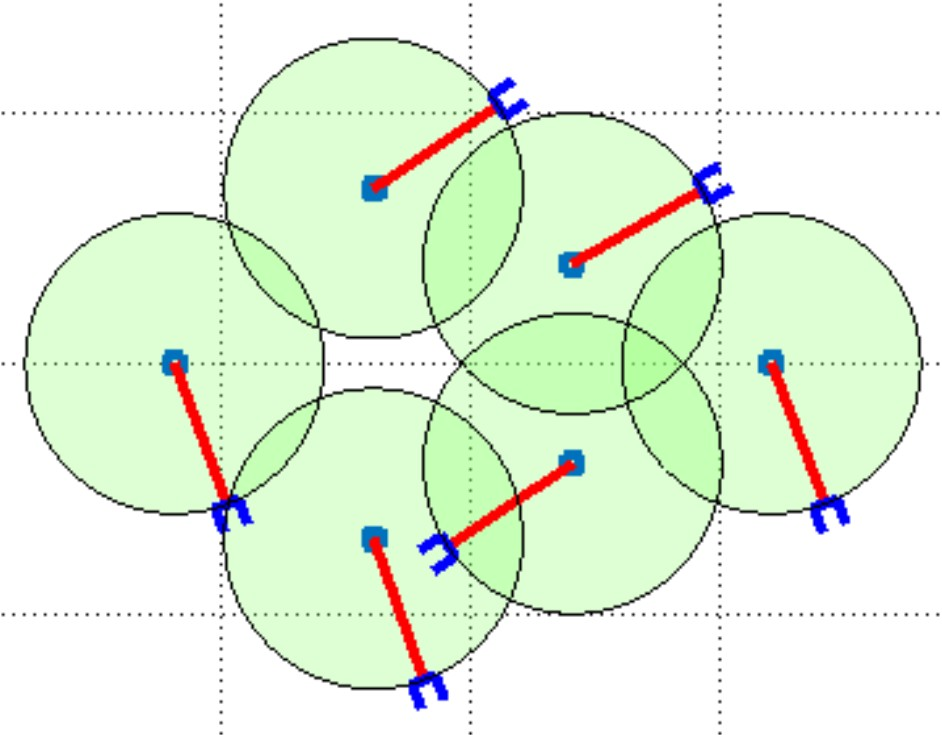
\includegraphics[width=\textwidth]{general_configuration}
        \caption{general configuration \\ ~~}
        \label{fig:general_configuration}
    \end{subfigure}
    ~~~~
    \begin{subfigure}[b]{0.4\textwidth}
        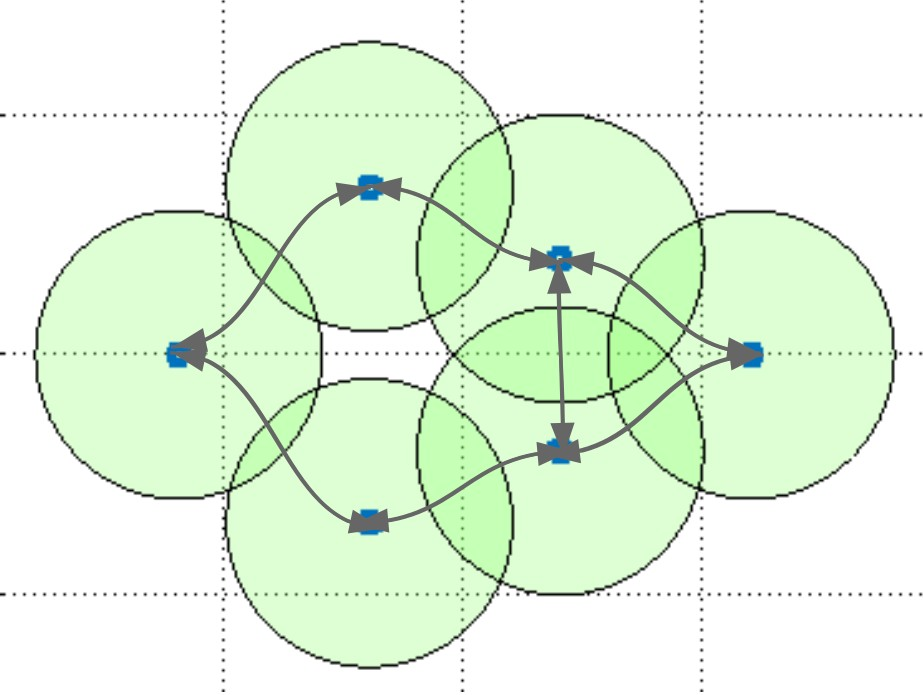
\includegraphics[width=\textwidth]{generated_graph}
        \caption{phase 1: generated connectivity graph}
        \label{fig:connectivity_graph}
    \end{subfigure}  
    
    \begin{subfigure}[b]{0.4\textwidth}
        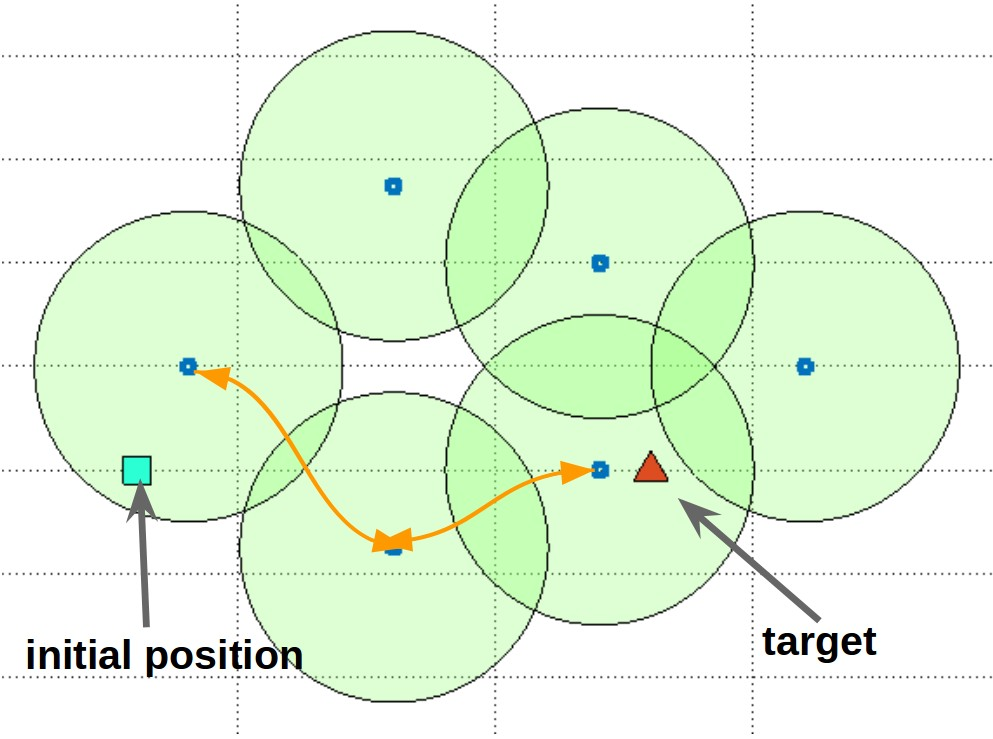
\includegraphics[width=\textwidth]{task_assignment}
        \caption{phase 2: Graph shortest path based on task properties }
        \label{fig:task_assignment}
    \end{subfigure}
    ~~~~
    \begin{subfigure}[b]{0.4\textwidth}
        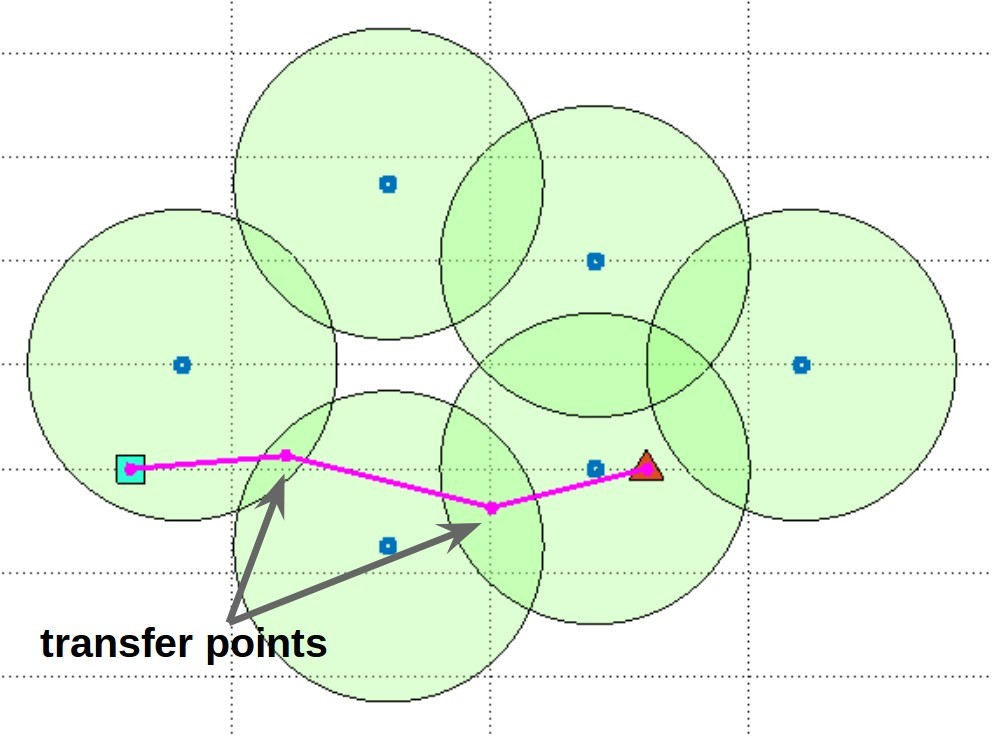
\includegraphics[width=\textwidth]{transfer_points}
        \caption{phase 3: calculating transfer points}
        \label{fig:transfer_points}
    \end{subfigure}
    \caption{Generating a sequence of arms and transfer points}\label{fig:animals}
\end{figure}

\subsubsection*{Search for Arm Sequence and Transfer Points}

One of the key component of our work is find any pair of arms sharing together a part of their workspace such that $W^i \cap W^j \neq \emptyset$. This fact gives an insight for any transfer that could appear. Representing this data is made by using a graph where nodes represents an arm workspace and arcs represents a shared workspace between two arms. It means that a setup consist of $M$ arms is interpreted by a graph with $M$ nodes. Adding the graph arcs is applied by 
going throw any possible combination of two arms and check whether together they share a part of their workspace. The generation of this graph will tentatively be called the \textit{connectivity graph}. An example illustration of such a graph is given in figure \ref{fig:connectivity_graph}.

By attributing the initial and goal position of the object ($B^{init}$ and $B^{goal}$) to one of the arms work space we can reason about the starting and final node in the \textit{connectivity graph}. At this point, any graph search would give a solution with a form of a sequence of arms index $\mathcal{S} = \langle s^1,...,s^k,...,s^K \rangle$ connected by their shared workspaces (as shown in figure \ref{fig:task_assignment}) such that:
\begin{equation}
B^{init} \in W^{\mathcal{S}(1)}
\end{equation}
\begin{equation}
B^{goal} \in W^{\mathcal{S}(K)}
\end{equation}
\begin{equation}
W^{\mathcal{S}(k)}\cap W^{\mathcal{S}(k+1)}\neq \emptyset
\end{equation}

To complete the algorithm first phase we still have to determine the positions of the \textit{transfer point series}. As shown in figure \ref{fig:transfer_points} we can detect that any \textit{transfer point} is located in the shared work space of any two successive arms in $\mathcal{S}$. Still, we have to determine the exact position in the shared work space. One option is to use a linear programming method to minimize the total length accepted by connecting any pair of successive \textit{transfer point} by a straight line. In our implementation we choose a more straight forward method and selected the center of area of the shared workspace.


\subsubsection*{The Search Algorithm}
Algorithm \ref{alg:main-loop} shows the main procedure for generating a solution. Here, lines 1-5 represents the first phase of the algorithm for calculating the transfer arms and transfer points where line 6 represent the motion planing phase. 

To generate an actual sequence that will apply the condition as in equations \eqref{eq:kinematic-feasible}-\eqref{eq:no-collision} we will have to go through the steps as written in algorithm \ref{alg:main-loop}. The rationale behind this algorithm is first to find a sequence of arms $S$ together with a series of $transfer~points$ $tp$ that will settle with equation \eqref{eq:consistant-sequence} (lines 1-5). Next, when $S$ and $tp$ was determined the guidelines for a motion plan was resolved, thus the second phase of the algorithm was launched (line 6) in order to calculate the sequence path that meet equations \eqref{eq:kinematic-feasible} and \eqref{eq:no-collision}. 

\begin{algorithm}
\caption{Main Loop} \label{alg:main-loop}
\begin{algorithmic}  [1] % the [1] is for numbering
\REQUIRE $B^{init},B^{goal},\mathcal{A}$
\ENSURE $\mathcal{Q}$
	\STATE $cg\leftarrow$ Generate $ConnectivityGraph\left(\mathcal{A}\right)$
	\STATE $W^{first}\leftarrow $ find($W^{first}$ such that $B^{init}\in W^{first}$)
	\STATE $W^{last}\leftarrow $ find($W^{last}$ such that $B^{goal}\in W^{last}$)
	\STATE $\mathcal{S}\leftarrow$ BFS$( cg,W^{first},W^{last})$ // generate ws sequence
	\STATE $TPS\leftarrow$ Calc $TransferPointsSeries\left(\mathcal{S},B^{init},B^{goal}\right)$
\STATE $\mathcal{T}^A \leftarrow CalcSequenceTrajectory( S,tp,q^{init})$
\end{algorithmic}
\end{algorithm}


\subsection{Multi Arm Motion Planning}
As stated, at this stage our goal is to calculate the arms path for each phase of the \textit{manipulation-path} represented by $\mathcal{T}^A$. We assume that each phase includes the following input parameters (and that the initial configuration of the total arms is known):

\begin{itemize}
	\item Index of the moving arm.
	\item Initial and goal positions of the arms gripper
\end{itemize}

These parameters directs us to find a motion planning solution for a multi robot system. As mentioned in section \ref{section:motion_planning} there is no formal strategy for calculating optimal nor complete trajectory for multi robots except for using \textit{centralized} methods that suffers from exponential complexity. The pattern that we will next describe is a method that is designed to find a solution oriented for robotic arms but may still be used for other systems. 

The fact that a \textit{centralized} method includes complete and optimal attributes is that it can handle local minima's (same as A*). Lack in such feature resolved in having no reasoning when: robot 2 obstructs the path of robot 1 where actually robot 1 obstructs the path of robot 2 that should clear the path for robot 1. A simple illustration is shown in figure \ref{fig:initial_configuration} with a case of 2 robotic arms having 1 DoF each. The task here is to move arm \#1 to the dashed line. Trying to do so with applying any motion plan on arm \#1 only will result with "no solution" answer. It is obvious that arm \#2 needs to clear the way and the only option is to move counter-clockwise (moving clockwise is impassible due to the obstacle). 



\begin{figure}[t]
    \centering
    \begin{subfigure}[b]{0.3\textwidth}
    		\centering
        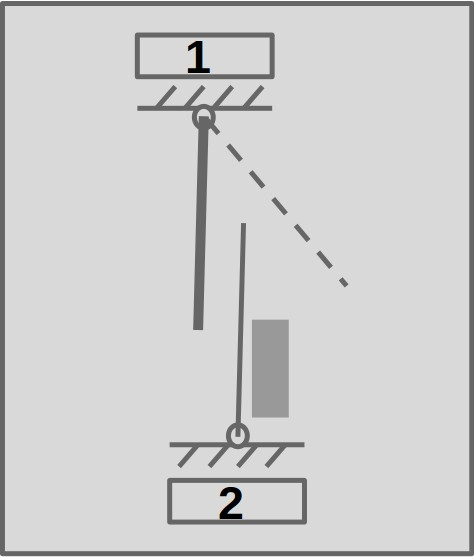
\includegraphics[width=0.8\textwidth]{initial_configuration}
        \caption{Initial configuration of the arms, goal of arm \#1 is dashed \\ }
        \label{fig:initial_configuration}
    \end{subfigure}
    ~
    \begin{subfigure}[b]{0.3\textwidth}
    		\centering
        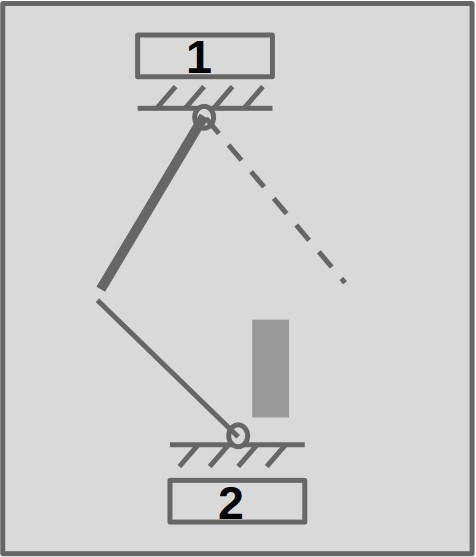
\includegraphics[width=0.8\textwidth]{breaking_point}
        \caption{A configuration of a "breaking point" from which the goal is reachable for a single arm task}
        \label{fig:breaking_point}
    \end{subfigure}  
    ~
    \begin{subfigure}[b]{0.3\textwidth}
    		\centering
        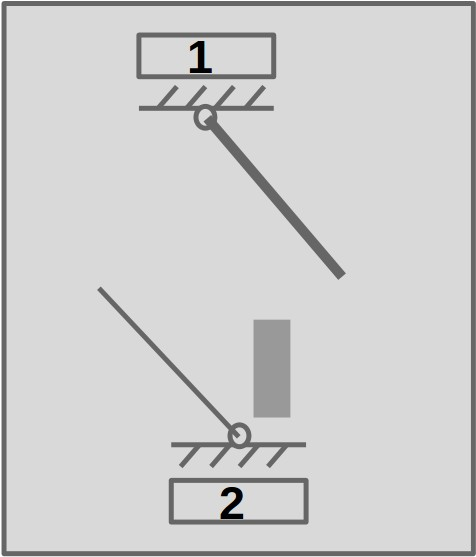
\includegraphics[width=0.8\textwidth]{final_configuration}
        \caption{Final configuration: goal achieved \\ ~~\\~~ }
        \label{fig:final_configuration}
    \end{subfigure}

    \caption{A multi arm problem configuration consist of 2 arms with 1 DoF each together with an obstacle (grey rectangle) that limits arm \#2 motion. In order to acheive the goal (figure c) a breaking point (figure b) must be acheived first. }\label{fig:local_minima_example}
\end{figure}




\newpage
\section{Research Program}

\begin{figure}[h]
	\centering
	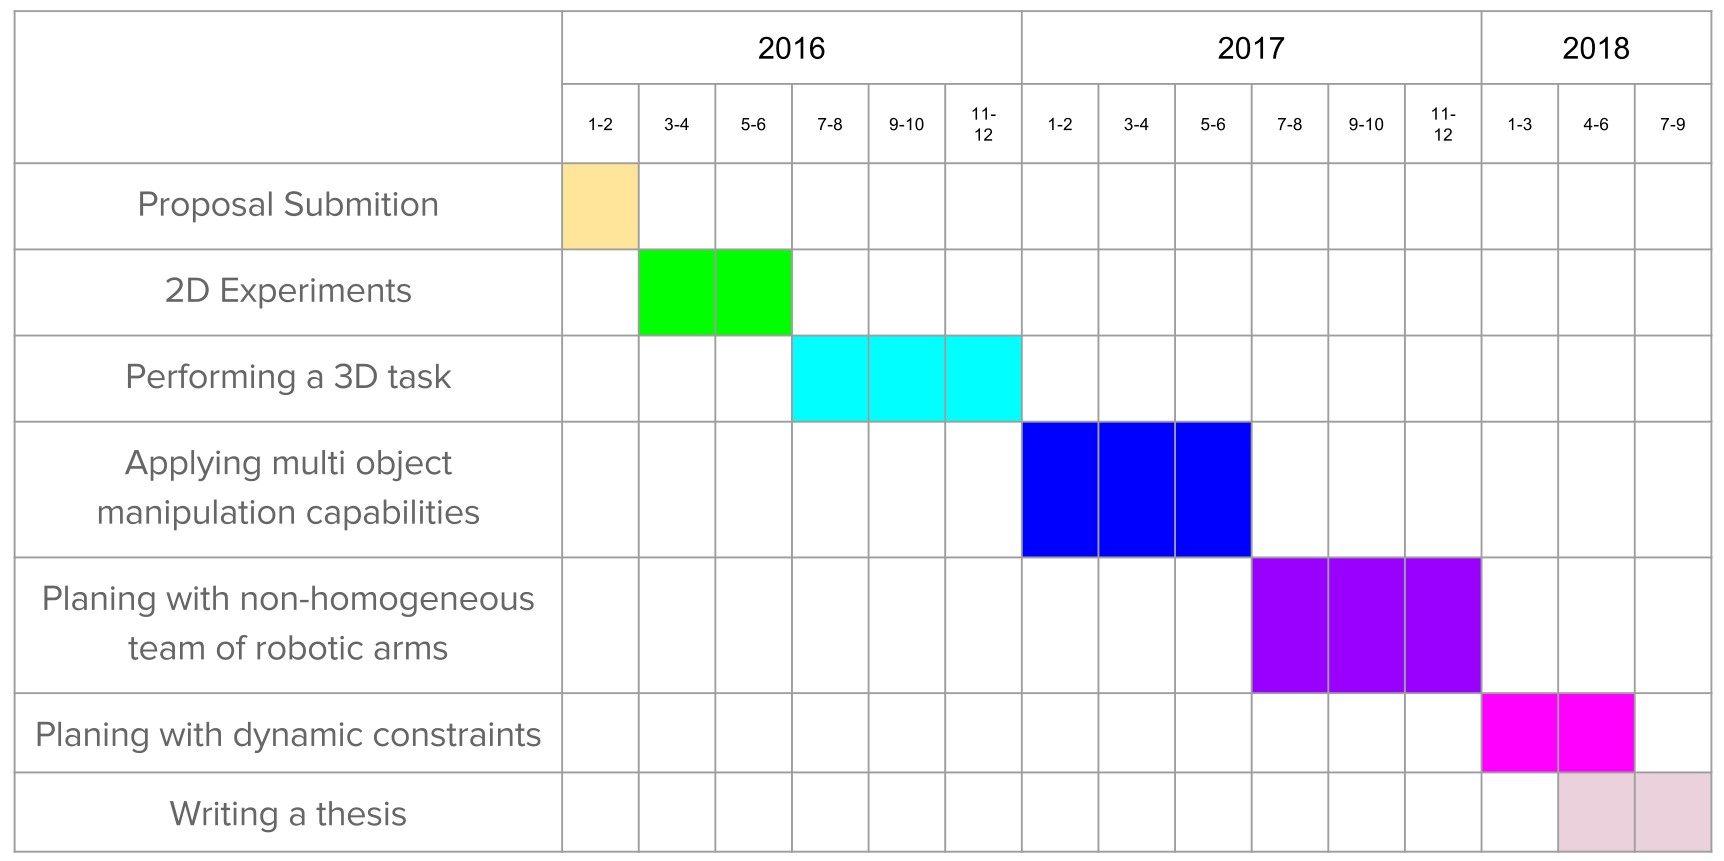
\includegraphics[width=\textwidth]{time_table}
	\caption{Time table}
\end{figure}

\newpage
\bibliography{proposal}

\end{document}